


\documentclass[conference]{IEEEtran}
\IEEEoverridecommandlockouts
% The preceding line is only needed to identify funding in the first footnote. If that is unneeded, please comment it out.
\usepackage{cite}
\usepackage{amsmath,amssymb,amsfonts}
\usepackage{algorithmic}
\usepackage{graphicx}
\usepackage{stfloats}
\usepackage{textcomp}
\usepackage{url}
\usepackage{xcolor}
\usepackage{multirow}
\def\BibTeX{{\rm B\kern-.05em{\sc i\kern-.025em b}\kern-.08em
    T\kern-.1667em\lower.7ex\hbox{E}\kern-.125emX}}
\begin{document}

% MDP 、MCRA添加参考文献
% index 部分结尾处要不要添加 。
%figure reports -> shows
% future work 改被动式
% 主动换被动
% 避免中式英语-结论部分

\title{HD-MCRA: Hierarchical Reach-Avoid Navigation for Quadruped Robots}

\author{\IEEEauthorblockN{1\textsuperscript{st} Given Name Surname}
\IEEEauthorblockA{\textit{dept. name of organization (of Aff.)} \\
\textit{name of organization (of Aff.)}\\
City, Country \\
email address or ORCID}
\and
\IEEEauthorblockN{2\textsuperscript{nd} Given Name Surname}
\IEEEauthorblockA{\textit{dept. name of organization (of Aff.)} \\
\textit{name of organization (of Aff.)}\\
City, Country \\
email address or ORCID}
\and
\IEEEauthorblockN{3\textsuperscript{rd} Given Name Surname}
\IEEEauthorblockA{\textit{dept. name of organization (of Aff.)} \\
\textit{name of organization (of Aff.)}\\
City, Country \\
email address or ORCID}
}

\maketitle
\bstctlcite{IEEEexample:BSTcontrol}

\begin{abstract}
Quadruped navigation in cluttered environments requires reaching target locations, avoiding unsafe regions throughout execution, and minimizing cumulative navigation cost. We formulate this task as a minimum-cost reach-avoid problem, which explicitly encodes goal reaching, safety preservation, and cost minimization within a unified trajectory-level objective. To make this formulation practical for quadruped robots, we propose HD-MCRA, a hierarchical framework that combines a frozen robust low-level velocity tracker with a budget-conditioned high-level reach-avoid policy. The low-level tracker induces a stable closed-loop abstraction for high-level planning, while data-driven conservative margins improve robustness in both budget feasibility and safety. Simulation and real-world experiments show that HD-MCRA achieves a better trade-off among task success, safety, budget feasibility, clearance, and navigation cost than representative baselines. 
\end{abstract}

\begin{IEEEkeywords}
quadruped robot, navigation, reach-avoid, hierarchical reinforcement learning, safe reinforcement learning
\end{IEEEkeywords}

\section{Introduction}
Recent advances in learning-based quadruped locomotion and agile navigation have substantially improved motion capability and terrain adaptation on physical robots \cite{DBLP:journals/scirobotics/HwangboWK020,DBLP:conf/rss/KumarFPM21,DBLP:journals/scirobotics/MikiLHWKH22,Hoeller2024}. As a result, the primary deployment bottleneck has shifted from low-level locomotion capability to high-level autonomous navigation in cluttered environments. In practical missions such as inspection, search and rescue, and security patrol, quadruped navigation must satisfy two hard requirements simultaneously: collision-free goal reaching and low execution cost under contact-rich execution and perception uncertainty.

Existing methods do not fully solve this problem. Classical planners such as DWA and D* Lite \cite{DBLP:journals/ram/FoxBT97,DBLP:conf/aaai/KoenigL02} rely on modeling and execution assumptions that are difficult to maintain on quadruped platforms. In contrast, many reinforcement learning approaches optimize weighted rewards or constrained objectives \cite{DBLP:conf/icml/AchiamHTA17,DBLP:conf/iclr/TesslerMM19,GuerrierFB24}, which either relax safe goal-reaching into a tunable preference or introduce sensitivity to constraint-threshold selection. Recent reachability-based methods provide a principled framework for encoding safety, liveness, and cost feasibility beyond additive rewards, including reach-avoid RL and minimum-cost reach-avoid (MCRA) formulations such as the budget-conditioned RC-PPO framework \cite{DBLP:conf/rss/HsuRTF21,DBLP:conf/nips/SoGF24,Ganai2024HJSurvey,GanaiGYHG23}. However, these formulations are typically developed under deterministic or simplified dynamics, whereas quadruped deployment involves stochastic execution mismatch.

To overcome these limitations, \emph{HD-MCRA} (\emph{Hierarchical Data-driven Minimum-Cost Reach-Avoid}) is proposed as a hierarchical MCRA framework with data-driven conservative margins for quadruped navigation. A robust low-level velocity tracker is first trained with PPO under domain randomization and then frozen to induce an approximately deterministic interface for high-level learning. On top of this interface, a high-level budget-conditioned reach-avoid policy is learned over low-dimensional velocity commands, and two data-driven conservative margins, $\alpha$ and $\delta$, are introduced to compensate for budget overrun and trajectory deviation. 

The main contributions are twofold: 1) quadruped navigation is formulated as an MCRA problem that explicitly encodes safe goal-reaching and cost minimization; and 2) a hierarchical MCRA framework with data-driven conservative margins is developed to make budget-conditioned MCRA learning practical for quadruped robots.

The remainder of this paper is organized as follows. Section II introduces the MCRA formulation for quadruped navigation. Section III presents the HD-MCRA framework and its learning procedure. Section IV evaluates the proposed method in simulation and real-world experiments. Section V concludes the paper.





















\section{Problem Formulation}
To formalize quadruped navigation in cluttered environments, the high-level decision-making process is modeled as a Markov decision process (MDP)
\begin{equation}
\mathcal{M}=\langle \mathcal{X}, \mathcal{U}^{\mathrm{high}}, P, c, \rho_0 \rangle
\end{equation}
where $\mathcal{X}$ denotes the high-level state space, $\mathcal{U}^{\mathrm{high}}$ denotes the action space of commanded base velocities, $P(\cdot|x_t,u_t)$ denotes the transition kernel, $c(x_t,u_t)$ denotes the instantaneous execution cost, and $\rho_0$ denotes the initial-state distribution.

Let $\mathcal{G}\subseteq\mathcal{X}$ denote the goal set and $\mathcal{F}\subseteq\mathcal{X}$ denote the unsafe set induced by collision or safety violation. Starting from an initial state $x_0$, the task is to find a policy $\pi$ and a free terminal time $T$ such that the robot reaches $\mathcal{G}$, avoids $\mathcal{F}$ throughout the trajectory, and minimizes the cumulative cost. Motivated by the deterministic MCRA formulation in \cite{DBLP:conf/nips/SoGF24}, a stochastic MCRA problem is considered for quadruped navigation:
\begin{align}
\min_{\pi,T}\quad & \sum_{t=0}^{T-1} c\!\left(x_t,\pi(x_t)\right) \label{eq:mcra_obj}\\
\mathrm{s.t.}\quad & x_T \in \mathcal{G}, \label{eq:mcra_goal}\\
& x_t \notin \mathcal{F},\quad \forall t\in\{0,\dots,T\}, \label{eq:mcra_safe}\\
& x_{t+1}\sim P\!\left(\cdot\mid x_t,\pi(x_t)\right). \label{eq:mcra_dyn}
\end{align}
The goal and unsafe sets are represented by two signed functions
$g:\mathcal{X}\rightarrow\mathbb{R}$ and $h:\mathcal{X}\rightarrow\mathbb{R}$ as
\begin{equation}
\mathcal{G} := \{x\in\mathcal{X}\mid g(x)\le 0\}
\end{equation}
\begin{equation}
\mathcal{F} := \{x\in\mathcal{X}\mid h(x)>0\}
\end{equation}
Unlike reward shaping, this formulation enforces goal-reaching and safety as trajectory-level constraints rather than soft preferences induced by weighted rewards. This distinction is important in quadruped navigation, where surrogate reward or CMDP objectives may not align with the actual objective of safe goal-reaching with minimum cumulative cost \cite{DBLP:conf/nips/SoGF24}.

RC-PPO recasts the MCRA problem as a reachability problem on an augmented state space \cite{DBLP:conf/nips/SoGF24}. This construction was developed for deterministic discrete-time dynamics of the form $x_{t+1}=f(x_t,u_t)$, rather than for the stochastic dynamics in \eqref{eq:mcra_dyn}. The deterministic augmented-state formulation is therefore briefly recalled below. 

The augmented state is defined as
\begin{equation}
\hat{x}_t=(x_t,y_t,z_t)\in \hat{\mathcal{X}}:=\mathcal{X}\times\{-1,1\}\times\mathbb{R}
\end{equation}
where $y_t$ is a binary safety indicator and $z_t$ is a remaining cost budget. The corresponding augmented dynamics are
\begin{equation}
\begin{aligned}
\hat{f}(x_t,y_t,z_t,u_t)
= \big(&f(x_t,u_t), \\
&\max\{I_{f(x_t,u_t)\in\mathcal{F}},y_t\}, \\
&z_t-c(x_t,u_t)\big)
\end{aligned}
\end{equation}
where $I_{b\in\mathcal{B}}$ is the shifted indicator. By construction, $z_t$ evolves as
\begin{equation}
z_{t+1}=z_0-\sum_{k=0}^{t} c(x_k,u_k)
\end{equation}
which means that $z_0$ serves as an upper bound on the cumulative cost incurred along the trajectory. Then the augmented goal function can be defined as
\begin{equation}
\hat{g}(x,y,z)=\max\{g(x),Cy,-z\}
\end{equation}
with augmented goal set
\begin{equation}
\begin{aligned}
\hat{\mathcal{G}}
&=\{\hat{x}\mid \hat{g}(\hat{x})\le 0\} \\
&=\{(x,y,z)\mid x\in\mathcal{G},\, y=-1,\, z\ge 0\}
\end{aligned}
\end{equation}
Under this construction, if the augmented state reaches the augmented goal set $\hat{\mathcal{G}}$, then the original system reaches the goal, remains safe along the whole trajectory, and does not exceed the prescribed budget \cite{DBLP:conf/nips/SoGF24}. Accordingly, the deterministic MCRA problem can be equivalently interpreted as searching for the least feasible initial budget
\begin{align}
\min_{\pi,z_0}\quad & z_0 \\
\mathrm{s.t.}\quad & \tilde{V}^{\pi}_{\hat{g}}(x_0,I_{x_0\in\mathcal{F}},z_0)\le 0,
\end{align}
where $\tilde{V}^{\pi}_{\hat{g}}$ is the reach value function on the augmented system.

However, this deterministic reformulation alone is insufficient for quadruped navigation, since real-world execution remains stochastic and can lead to budget overruns and trajectory deviations. Bridging this gap requires a quadruped-specific nominal closed-loop abstraction together with conservative corrections to account for residual mismatch, which motivates the HD-MCRA framework introduced next.







\section{HD-MCRA}
\subsection{Framework Overview}
As shown in Figure~\ref{fig:framework_overview}, HD-MCRA consists of a frozen low-level locomotion controller, a budget-conditioned high-level planner, and data-driven conservative margins. This hierarchical structure reduces the action dimensionality of the navigation problem, preserves locomotion feasibility, and provides a more stationary closed-loop system for high-level MCRA learning. The frozen low-level tracker serves as a stable motion interface, while the conservative margins $\alpha$ and $\delta$ further compensate for residual mismatch in cost and safety.

\begin{figure}[t]
\centering
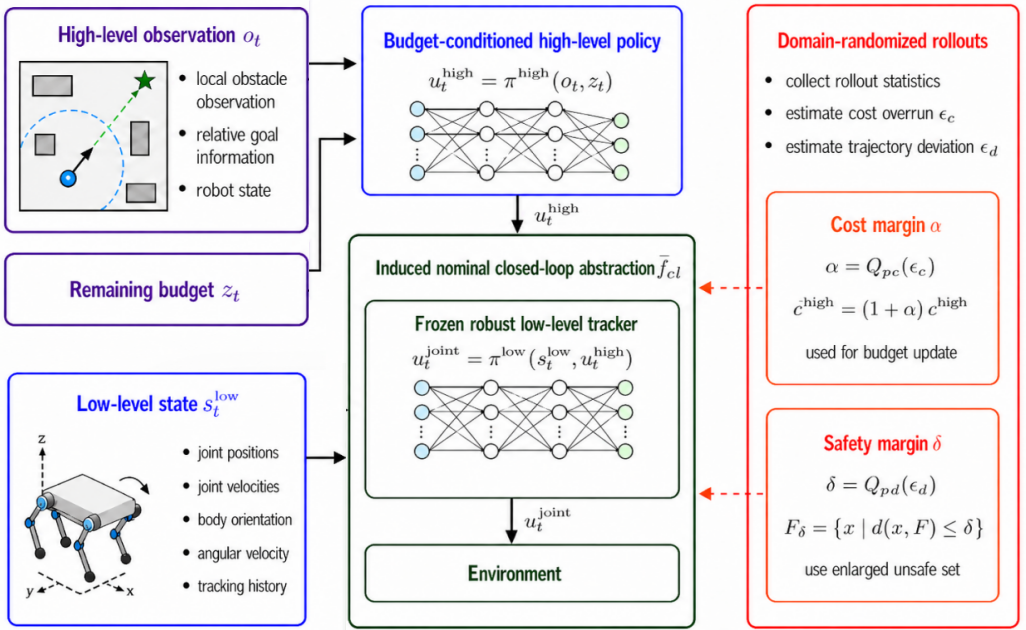
\includegraphics[width=\columnwidth]{../../images/framework_overview.png}
\caption{Overview of the HD-MCRA framework.}
\label{fig:framework_overview}
\end{figure}


Formally, let the overall policy be written as
\begin{equation}
u_t^{\mathrm{joint}}
=\pi^{\mathrm{low}}\big(s_t^{\mathrm{low}},u_t^{\mathrm{high}}\big)
\end{equation}
\begin{equation}
u_t^{\mathrm{high}}
=\pi^{\mathrm{high}}(o_t,z_t)
\end{equation}
where $o_t$ denotes the high-level observation, $u_t^{\mathrm{high}}$ denotes the commanded base velocity, $s_t^{\mathrm{low}}$ denotes the low-level locomotion state, and $u_t^{\mathrm{joint}}$ denotes the final joint-level control action. This factorization allows the navigation problem to be solved in a lower-dimensional action space while preserving the physical feasibility of locomotion execution.

\subsection{Hierarchical Budgeted Policy Learning}

The low-level controller maps proprioceptive observations to actuator commands to track high-level velocity commands while preserving locomotion stability. Its state is $s_t^{\mathrm{low}} \in \mathcal{S}^{\mathrm{low}}$, which includes joint positions, joint velocities, body orientation, angular velocity, and recent tracking information, and its action is the joint-level command $u_t^{\mathrm{joint}} \in \mathcal{U}^{\mathrm{joint}}$. Given a commanded base velocity
\begin{equation}
u_t^{\mathrm{high}} = \big[v_{x,t}^{\ast}, v_{y,t}^{\ast}, \omega_{z,t}^{\ast}\big]^{\top}
\end{equation}
the controller aims to minimize tracking error while maintaining stable motion.

This controller is trained with PPO under domain randomization \cite{DBLP:journals/corr/SchulmanWDRK17,DBLP:conf/iros/TobinFRSZA17}. Let $\bar{u}_t^{\mathrm{body}}=[v_{x,t},v_{y,t},\omega_{z,t}]^{\top}$ denote the realized body velocity. The reward combines velocity-tracking, control-smoothness, and posture-stability terms:
\begin{equation}
\begin{aligned}
r_t^{\mathrm{low}}
=\,&-\lambda_v \left\| \bar{u}_t^{\mathrm{body}}-u_t^{\mathrm{high}} \right\|_2^2 \\
&-\lambda_u \left\| u_t^{\mathrm{joint}} \right\|_2^2 -\lambda_p \phi_t^{\mathrm{stab}}
\end{aligned}
\end{equation}
where $\phi_t^{\mathrm{stab}}$ penalizes unstable motions such as excessive roll, pitch, or slippage. Randomizing dynamics and terrain parameters improves robustness, and the trained $\pi^{\mathrm{low}}$ is frozen before high-level learning.

With this motion interface fixed, the high-level process induces a reduced closed-loop transition kernel $P_{\mathrm{cl}}(\cdot\mid x_t,u_t^{\mathrm{high}})$. For high-level training, this kernel is approximated by a nominal closed-loop map, yielding
\begin{equation}
x_{t+1}=\bar{f}_{\mathrm{cl}}\!\left(x_t,u_t^{\mathrm{high}}\right)
\end{equation}
where $\bar{f}_{\mathrm{cl}}$ denotes the nominal closed-loop abstraction obtained by composing the robot dynamics with the frozen low-level tracker. Domain-randomized rollouts indicate that this induced kernel is substantially more concentrated than the transition distribution produced by end-to-end joint-space control, making the nominal abstraction useful at the navigation level.

On top of this fixed interface, the high-level policy solves the navigation problem using the MCRA formulation introduced in Section II. Let the high-level observation be $o_t \in \mathcal{O}$, which contains local LiDAR-based obstacle information, relative goal information, and the robot's state. The high-level action is the commanded base velocity
\begin{equation}
u_t^{\mathrm{high}}=\pi^{\mathrm{high}}(o_t,z_t)
\end{equation}
where $z_t$ is the remaining budget variable.

The high-level policy is conditioned on the remaining budget $z_t$, so that one policy can adapt to different cost-feasibility levels. Intuitively, larger budgets permit more conservative maneuvers, whereas tighter budgets encourage shorter and more efficient motion, provided that safety is preserved.

The high-level objective is to learn a policy that safely reaches the goal within feasible cost budgets while enabling the search for the minimum feasible initial budget:
\begin{align}
\min_{\pi^{\mathrm{high}}, z_0}\quad & z_0 \\
\mathrm{s.t.}\quad &
x_T \in \mathcal{G}, \;
x_t \notin \mathcal{F}, \ \forall t\le T .
\end{align}

\noindent\textbf{Assumption 1 (Concentrated closed-loop abstraction).}
With the low-level tracker frozen, the induced high-level closed-loop transition kernel is concentrated around $\bar{f}_{\mathrm{cl}}$. In particular, the one-step deviation
\(
e_t:=x_{t+1}-\bar{f}_{\mathrm{cl}}(x_t,u_t^{\mathrm{high}})
\)
and the relative cost overrun ratio admit bounded upper quantiles under domain-randomized rollouts.

\subsection{Data-driven Robustness Margins}

Despite the concentrated closed-loop abstraction, residual mismatch remains during real-world quadruped execution. This mismatch mainly manifests as cost overruns and trajectory deviations, which can respectively violate budget feasibility and reduce safety margins.

To account for this residual mismatch, two conservative margins are introduced: a \emph{cost margin} $\alpha$ for budget robustness and a \emph{safety margin} $\delta$ for geometric robustness.

The cost margin inflates the effective running cost:
\begin{equation}
\tilde{c}^{\mathrm{high}}(x_t,u_t^{\mathrm{high}})
=(1+\alpha)\, c^{\mathrm{high}}(x_t,u_t^{\mathrm{high}})
\end{equation}
so that the high-level budget update becomes
\begin{equation}
z_{t+1}=z_t-\tilde{c}^{\mathrm{high}}(x_t,u_t^{\mathrm{high}})
\end{equation}
This design reserves additional budget against execution-induced cost overruns. The margin $\alpha$ is estimated from the upper quantiles of the empirical cost-overrun distribution:
\begin{equation}
\alpha = Q_{p_c}(\varepsilon_c)
\end{equation}
where $\varepsilon_c$ denotes the relative cost overrun ratio between actual and nominal execution.

The safety margin enlarges the unsafe set as
\begin{equation}
\mathcal{F}_{\delta}=\{x\in\mathcal{X}\mid d(x,\mathcal{F})\le \delta\}
\end{equation}
where $d(x,\mathcal{F})$ denotes the distance from the state to the unsafe set. Replacing $\mathcal{F}$ with $\mathcal{F}_{\delta}$ encourages greater obstacle clearance and improves robustness to trajectory deviations. The margin $\delta$ is estimated from the upper quantiles of the empirical trajectory-deviation distribution:
\begin{equation}
\delta = Q_{p_d}(\varepsilon_d)
\end{equation}
where $\varepsilon_d$ denotes the deviation from the nominal body path. Here, $Q_p(\cdot)$ denotes the empirical $p$-quantile. The resulting surrogate problem is solved on the nominal closed-loop abstraction $\bar{f}_{\mathrm{cl}}$ with inflated running cost $\tilde{c}^{\mathrm{high}}$ and enlarged unsafe set $\mathcal{F}_{\delta}$.

\noindent\textbf{Remark 1 (Quantile-based robustness intuition).}
If a nominal trajectory generated by $\bar{f}_{\mathrm{cl}}$ reaches $\mathcal{G}$ while remaining outside $\mathcal{F}_{\delta}$ and satisfying the inflated budget update with $\tilde{c}^{\mathrm{high}}$, then the realized trajectory remains safe and budget-feasible whenever the trajectory deviation and cost overrun stay within the empirical quantile ranges used to define $\delta$ and $\alpha$. 

\subsection{Two-phase Solver}

Under this robustified formulation, the high-level policy is trained using a two-phase RL procedure. In \emph{Phase I}, a stochastic policy $\pi_\theta^{\mathrm{high}}(u\mid o,z)$ is trained together with a reachability critic on the augmented state $\hat{x}_t=(x_t,y_t,z_t)$. On the closed-loop abstraction, the critic is trained with the discounted reachability target
\begin{equation}
\begin{aligned}
\tilde{V}_{\psi}(\hat{x}_t)
=\,&(1-\gamma)\hat{g}(\hat{x}_t) \\
&+\,\gamma\, \mathbb{E}\!\left[
\min\!\left\{\hat{g}(\hat{x}_t),\tilde{V}_{\psi}(\hat{x}_{t+1})\right\}
\right]
\end{aligned}
\end{equation}
where $\hat{g}(x,y,z)=\max\{g(x),Cy,-z\}$ and $\hat{x}_{t+1}$ is generated by $\bar{f}_{\mathrm{cl}}$. During training, the initial budget $z_0$ is sampled from a prescribed interval $[z_{\min},z_{\max}]$.

In \emph{Phase II}, the stochastic actor is converted into a deterministic deployment policy using its mean action, and the value function is re-evaluated under the uncertainty-aware model defined by $\tilde{c}^{\mathrm{high}}$ and $\mathcal{F}_{\delta}$. The minimum feasible initial budget is then obtained by a one-dimensional search over $z_0$ for the start state or start-state distribution.




























\section{Experiments and Results}

\subsection{Experimental Setup}

Experiments were conducted on quadruped navigation tasks in cluttered environments, with three levels of difficulty: moderately cluttered scenes, narrow passages, and densely obstructed scenes.

We compare HD-MCRA with a reach-avoid baseline (RA) \cite{DBLP:conf/rss/HsuRTF21}, an MCRA baseline (RC-PPO) \cite{DBLP:conf/nips/SoGF24}, reward-shaped PPO, and CPPO with two safety weights ($\beta_L,\beta_H$). For a controlled comparison, all methods were evaluated using the same high-level observations, commanded-velocity action interface, frozen low-level tracker, and training/evaluation maps \cite{DBLP:conf/icml/AchiamHTA17,DBLP:conf/iclr/TesslerMM19,GuerrierFB24,MikiLWH24,DBLP:conf/icra/WeerakoonSEM24}. Performance is measured by Success Rate (SR), Collision Rate (CR), Average Cost, Budget Violation Rate (BVR), and Minimum Clearance (MC).

\subsection{Baseline Comparison}

Figure~\ref{fig:metrics_grid_single_column} shows the scenario-wise comparison in terms of SR, CR, Average Cost, and MC. Table~\ref{tab:main_result} summarizes the average performance over the three scenarios and also reports BVR.

\begin{figure}[t]
\centering
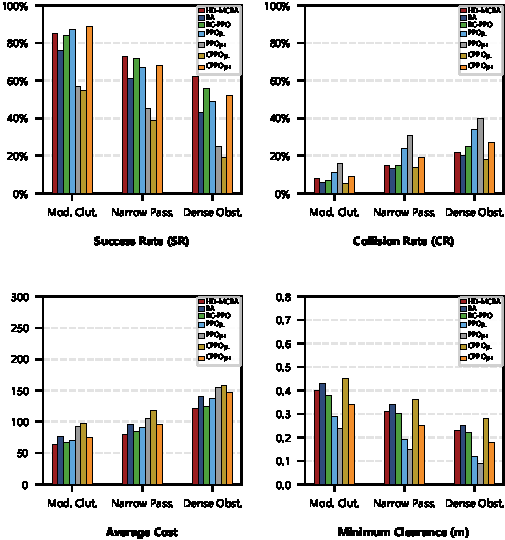
\includegraphics[width=\columnwidth]{../../images/figure_metrics_grid_single_column_v3}
\caption{Performance comparison across three navigation scenarios.}
\label{fig:metrics_grid_single_column}
\end{figure}


\begin{table}[t]
\caption{Average performance over the three scenarios.}
\label{tab:main_result}
\centering
\resizebox{\columnwidth}{!}{%
\begin{tabular}{lccccc}
\hline
Method & SR (\%) $\uparrow$ & CR (\%) $\downarrow$ & Cost $\downarrow$ & BVR (\%) $\downarrow$ & MC (m) $\uparrow$ \\
\hline
HD-MCRA & 73.3 & 15.0 & 88.3 & 9.0 & 0.31 \\
RA & 60.0 & 13.0 & 104.0 & 20.0 & 0.34 \\
RC-PPO & 70.7 & 15.7 & 91.7 & 14.0 & 0.30 \\
PPO$_{\beta L}$ & 67.7 & 23.0 & 99.7 & 20.7 & 0.20 \\
PPO$_{\beta H}$ & 42.3 & 29.0 & 117.0 & 27.0 & 0.16 \\
CPPO$_{\beta L}$ & 37.7 & 12.3 & 124.7 & 22.3 & 0.36 \\
CPPO$_{\beta H}$ & 69.7 & 18.3 & 105.7 & 17.0 & 0.26 \\
\hline
\end{tabular}}
\end{table}

Figure~\ref{fig:metrics_grid_single_column} and Table~\ref{tab:main_result} indicate that HD-MCRA achieves the most balanced overall performance across task completion, safety, budget feasibility, and efficiency in the three scenarios. Relative to RA, HD-MCRA achieves a higher success rate and lower cost while maintaining comparable safety. Compared with RC-PPO, HD-MCRA further improves budget feasibility and slightly increases minimum clearance, while also attaining the best average success rate. The PPO/CPPO baselines exhibit the usual trade-off: some settings remain competitive in easier scenes or improve clearance, but none matches HD-MCRA in terms of success, budget feasibility, and efficiency simultaneously.

\subsection{Budget Feasibility Analysis}

To evaluate budget sensitivity, we swept the normalized initial budget $z_0/z_{\mathrm{ref}}$ over $\{0.80,0.85,0.90,0.96,1.00,1.05,1.12,1.20\}$, where $z_{\mathrm{ref}}$ denotes a scenario-dependent reference feasible budget. Figure~\ref{fig:budget_sweep} reports the resulting SR, CR, BVR, and navigation cost curves for RA, RC-PPO, and HD-MCRA.

\begin{figure}[t]
\centering
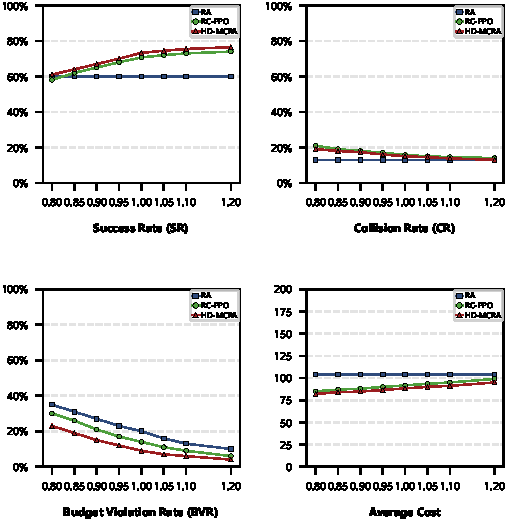
\includegraphics[width=\columnwidth]{../../images/figure_budget_sweep_v3}
\caption{Budget-response curves under normalized initial budgets.}
\label{fig:budget_sweep}
\end{figure}


RA is largely budget-agnostic: its SR, CR, and Average Cost remain almost unchanged across the sweep, and only BVR decreases as the budget is relaxed. In contrast, RC-PPO and HD-MCRA exhibit clear budget-response behavior, achieving higher SR and lower CR and BVR as the budget increases. HD-MCRA remains more reliable than RC-PPO even under tight budgets: at $z_0/z_{\mathrm{ref}}=0.90$, it achieves $66.8\%$ SR with $14.7\%$ BVR, whereas RC-PPO requires a larger budget to achieve comparable feasibility.

To compare budget feasibility across methods, we define the least feasible initial budget
\begin{equation}
\begin{aligned}
z_0^\star
= \min \Big\{ z_0 \;\Big|\; &\mathrm{SR}\ge 60\%,\; \mathrm{CR}\le 20\%, \\
&\mathrm{BVR}\le 15\% \Big\}
\end{aligned}
\end{equation}
where the criteria are evaluated on the complete test set. For methods without budget conditioning, such as RA, $z_0^\star$ is still evaluated by checking whether the realized trajectories satisfy the same budget-feasibility criteria under a given budget threshold. Table~\ref{tab:min_budget} shows that HD-MCRA achieves the smallest feasible budget, $z_0^\star/z_{\mathrm{ref}}=0.90$, compared with $0.96$ for RC-PPO and $1.12$ for RA. This indicates that budget conditioning is necessary for cost-feasible navigation and that the conservative margins improve robustness under execution uncertainty.

\begin{table}[t]
\caption{Search result for the minimum feasible normalized initial budget.}
\label{tab:min_budget}
\centering
\resizebox{\columnwidth}{!}{%
\begin{tabular}{lcccc}
\hline
Method & $z_0^\star / z_{\mathrm{ref}}$ $\downarrow$ & SR@${z_0^\star}$ (\%) $\uparrow$ & CR@${z_0^\star}$ (\%) $\downarrow$ & BVR@${z_0^\star}$ (\%) $\downarrow$ \\
\hline
HD-MCRA & 0.90 & 66.8 & 17.6 & 14.7 \\
RC-PPO & 0.96 & 62.9 & 18.8 & 14.9 \\
RA & 1.12 & 60.5 & 13.7 & 14.4 \\
\hline
\end{tabular}}
\end{table}

Figure~\ref{fig:budget_sweep} and Table~\ref{tab:min_budget} show that RA does not adapt to budget, RC-PPO captures the benefit of budget conditioning, and HD-MCRA reaches feasibility at the smallest budget.

\subsection{Ablation Study}

Ablation studies were conducted on the hierarchical structure and the conservative margins $\alpha$ and $\delta$. The compared variants are the full HD-MCRA framework, w/o Hierarchy, w/o $\alpha$, w/o $\delta$, and w/o $\alpha,\delta$. Since this study uses a separate evaluation batch, the values in Table~\ref{tab:ablation} are intended for within-table comparison only.

\begin{table}[t]
\caption{Ablation study on hierarchy and conservative margins.}
\label{tab:ablation}
\centering
\resizebox{\columnwidth}{!}{%
\begin{tabular}{lccccc}
\hline
Variant & SR (\%) $\uparrow$ & CR (\%) $\downarrow$ & Cost $\downarrow$ & BVR (\%) $\downarrow$ & MC (m) $\uparrow$ \\
\hline
w/o Hierarchy & 47.9 & 38.8 & 116.7 & 31.5 & 0.11 \\
w/o $\alpha$ & 67.2 & 19.8 & 80.6 & 22.4 & 0.29 \\
w/o $\delta$ & 64.8 & 26.3 & 77.2 & 13.8 & 0.19 \\
w/o $\alpha,\delta$ & 62.9 & 29.4 & 87.6 & 25.8 & 0.16 \\
HD-MCRA (full) & 70.8 & 18.6 & 71.3 & 11.2 & 0.32 \\
\hline
\end{tabular}}
\end{table}

Table~\ref{tab:ablation} shows that removing the hierarchy causes the largest overall degradation. Removing $\alpha$ mainly hurts budget feasibility, whereas removing $\delta$ mainly hurts safety and clearance. Removing both margins further degrades performance, confirming the complementary roles of the hierarchy and the two margins.

\subsection{Physical Robot Experiments}

The learned HD-MCRA policy was deployed on a Unitree Go2 robot in a cluttered office environment containing chairs, narrow passages, and moving obstacles. In one representative setup, a chair-defined passage was created whose width was only about $0.3\,\mathrm{m}$ larger than the robot. The chairs were placed in an alternating left-front, right-front, and left-front pattern, requiring the robot to execute consecutive turning maneuvers. A moving obstacle was further introduced near the goal region to test reactive avoidance under real-world execution mismatch.

For a start-to-goal distance of approximately $15\,\mathrm{m}$, the robot completed four out of five autonomous navigation trials successfully. In the successful trials, it stopped and avoided the moving obstacle effectively while maintaining stable locomotion. Figure~\ref{fig:office_sequence} shows a representative deployment sequence.

\begin{figure}[!t]
\centering
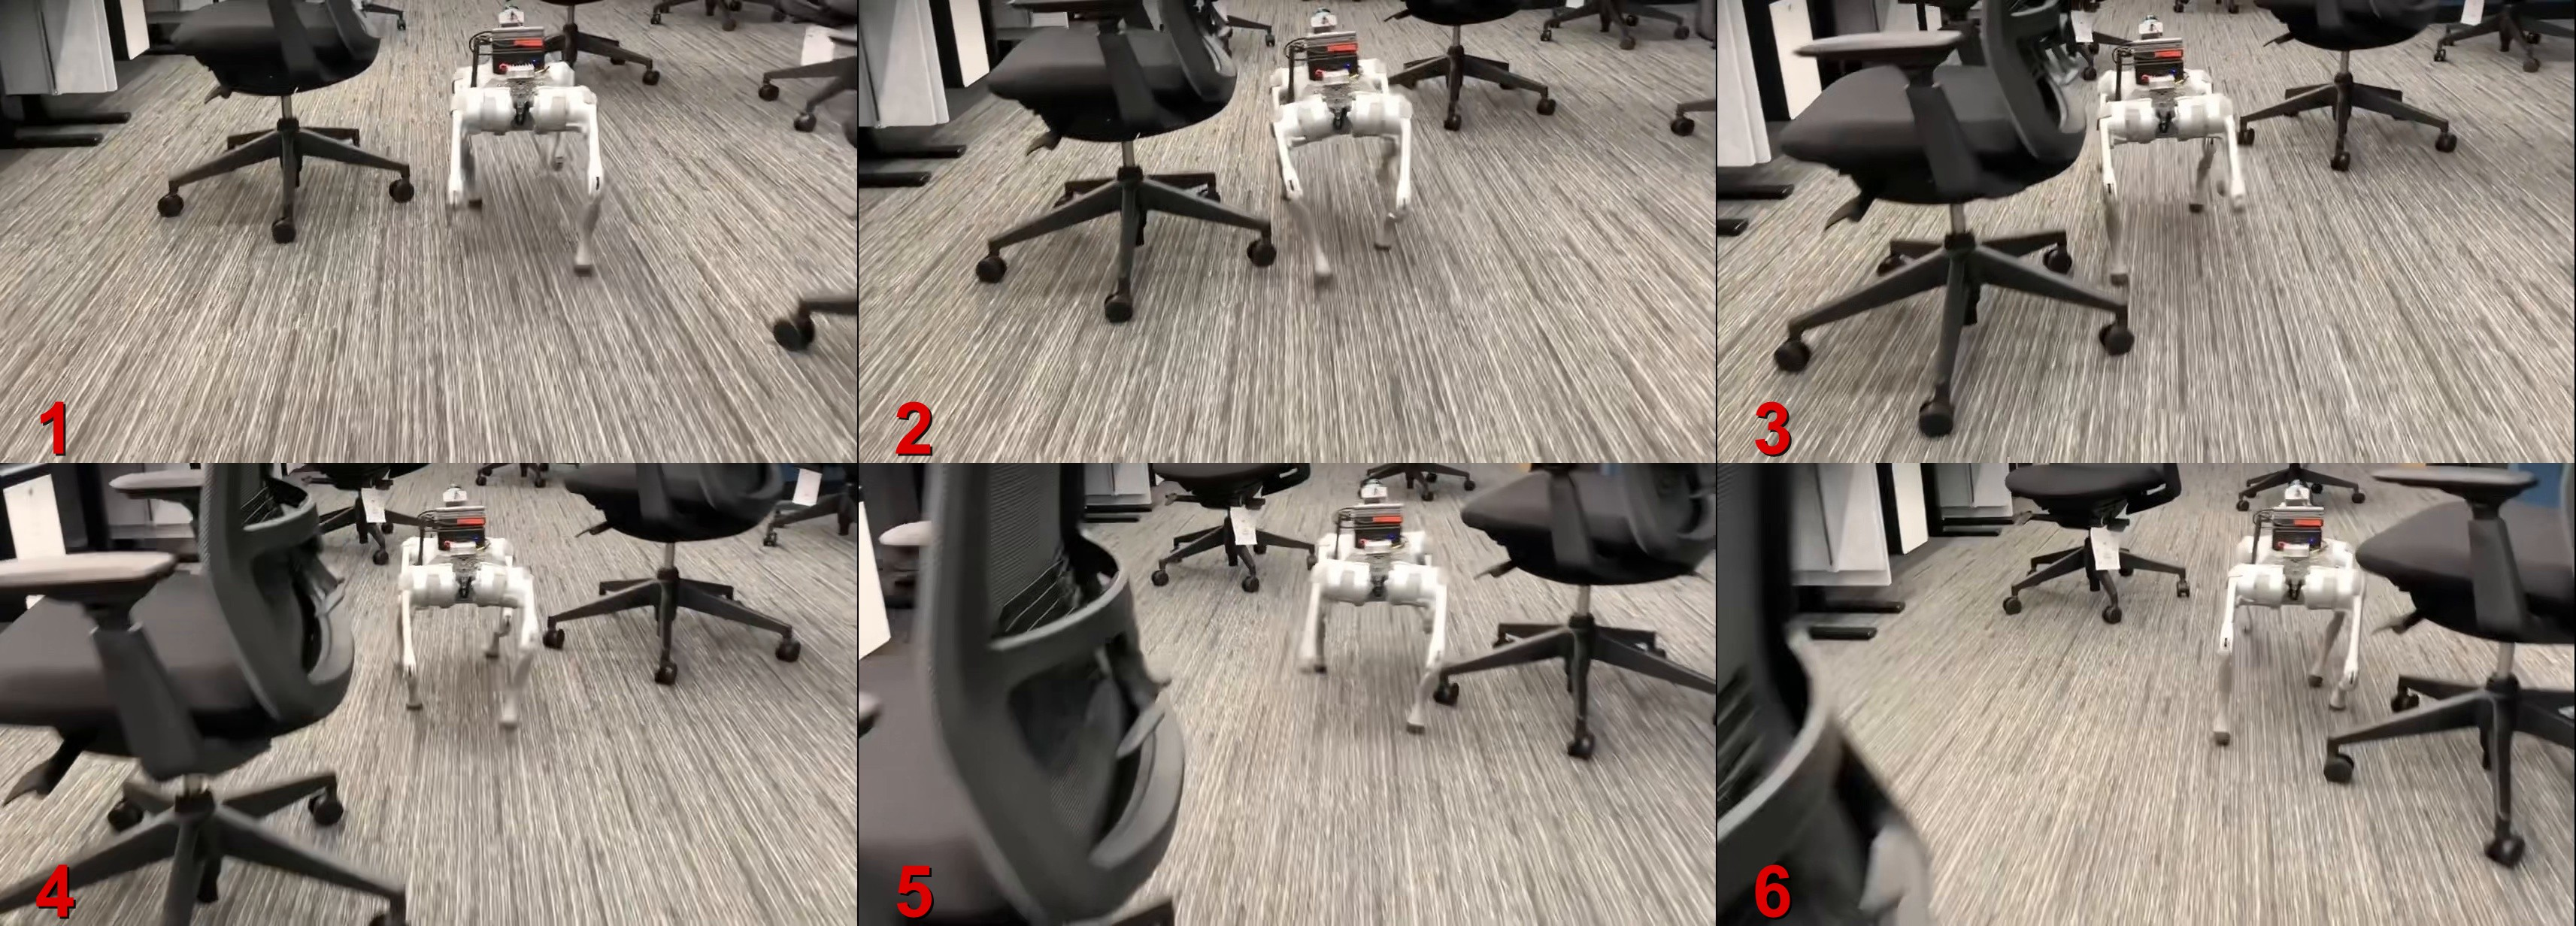
\includegraphics[width=\columnwidth]{../../images/office_sequence_candidate_A_numbered.jpg}
\caption{Real-world deployment in a cluttered office environment.}
\label{fig:office_sequence}
\end{figure}

In a second office setup, chair obstacles were densely placed in a wider corridor so that the shortest route passed through a noticeably narrower passage than alternative longer routes. The robot consistently selected this shorter feasible route and avoided collisions, indicating that the learned policy preferred efficient navigation while respecting local obstacle constraints. Figure~\ref{fig:office_shortest_path} shows a representative sequence from this shortest-path deployment.

\begin{figure}[!t]
\centering
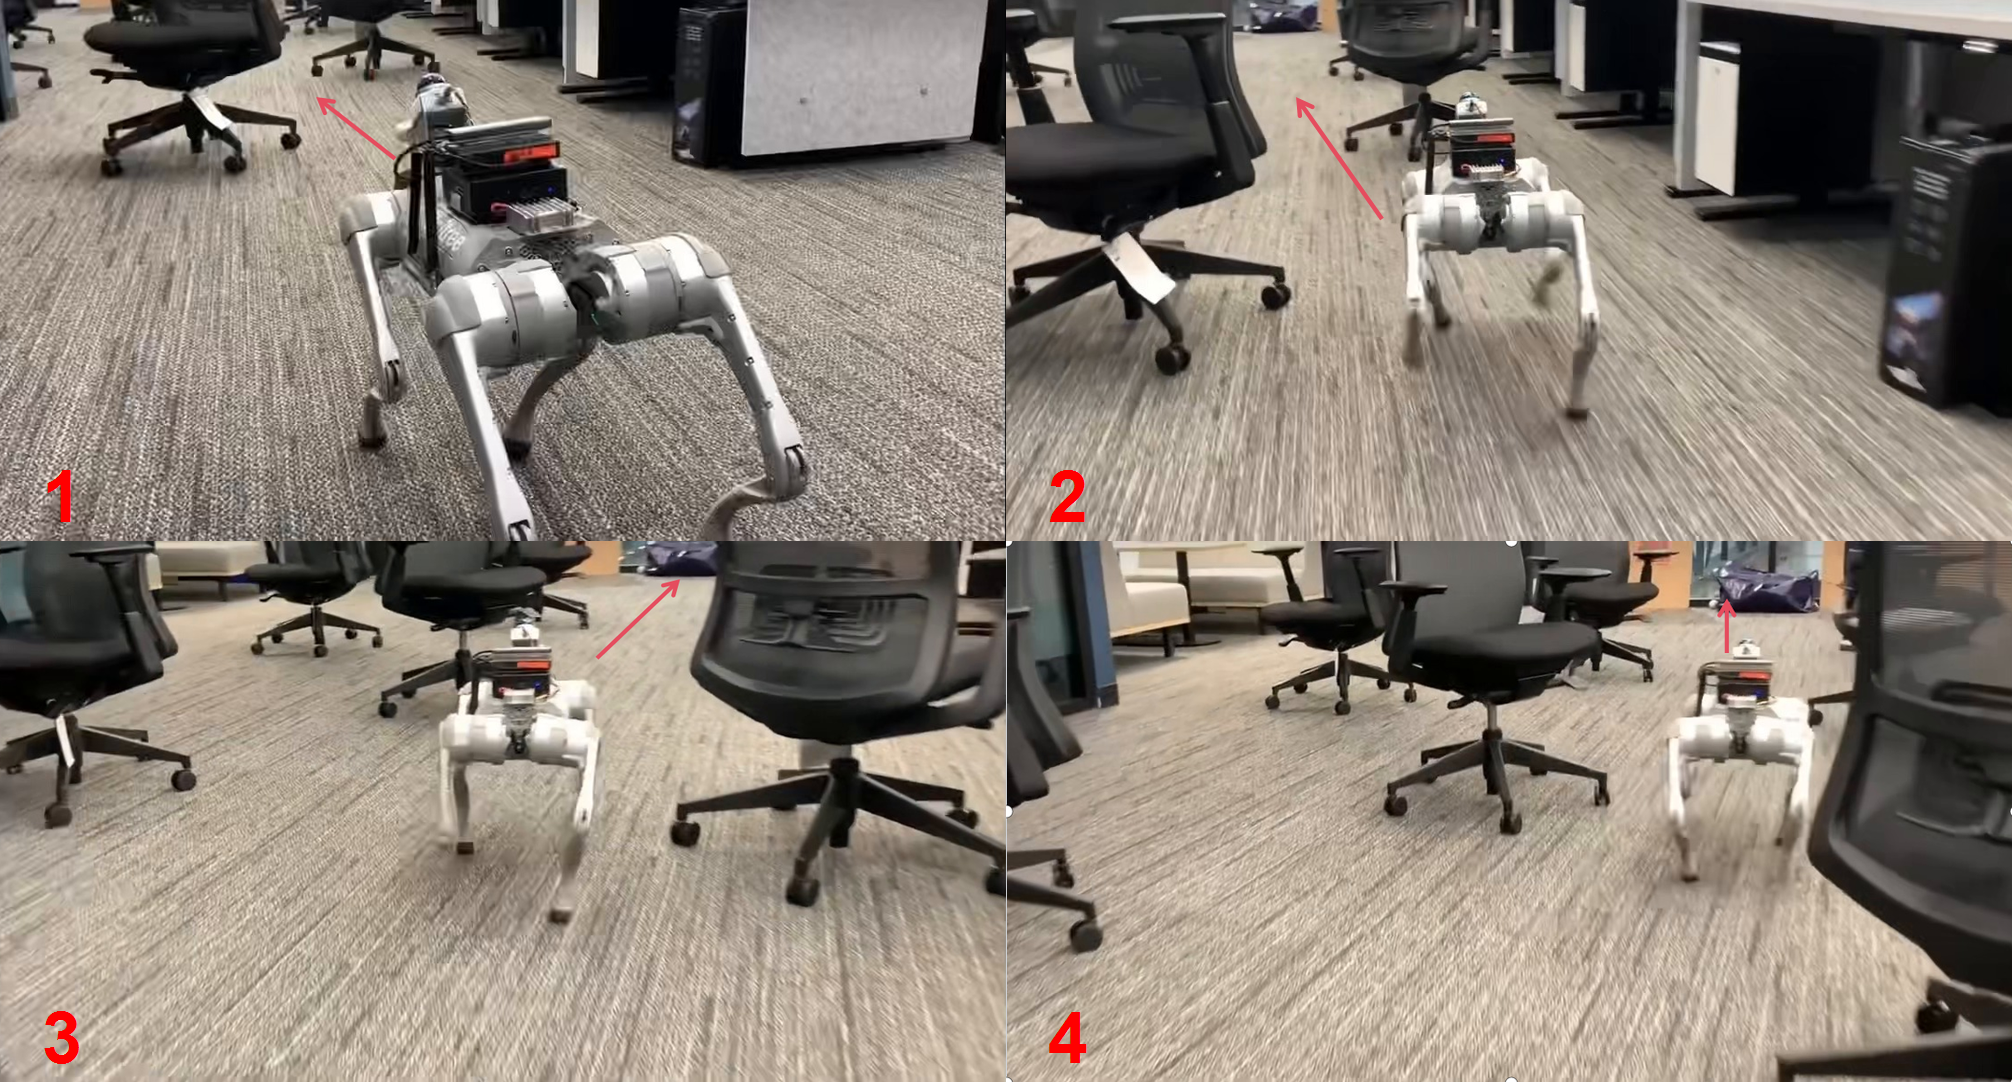
\includegraphics[width=\columnwidth]{../../images/office_shortest_path_strip_numbered.png}
\caption{Representative real-world deployment sequence in the shortest-path scenario.}
\label{fig:office_shortest_path}
\end{figure}

The observed failure case occurred when one of the quadruped's feet contacted a chair leg. This failure is likely due to the limited geometric saliency of narrow structures such as chair legs, together with residual mismatch during real-world execution. In particular, small trajectory deviations, body sway, or sensing latency can reduce the effective clearance near chair legs even when the nominal high-level path remains collision-free.




















\section{Conclusion}

This paper formulated quadruped navigation as an MCRA problem and proposed \emph{HD-MCRA}, which combines a frozen low-level tracker, a nominal closed-loop abstraction, a budget-conditioned high-level policy, and conservative cost and safety corrections. This design makes augmented-state MCRA practical for quadruped navigation and achieves a better trade-off among success, safety, budget feasibility, and efficiency than the evaluated baselines. An important direction for future work is to develop a theoretically grounded MCRA framework for stochastic quadruped navigation beyond the current engineering-oriented robust design.

\bibliographystyle{IEEEtran}
\bibliography{references}









\end{document}
